\documentclass{beamer}

%
% Choose how your presentation looks.
%
% For more themes, color themes and font themes, see:
% http://deic.uab.es/~iblanes/beamer_gallery/index_by_theme.html
%
\mode<presentation>
{
  \usetheme{default}      % or try Darmstadt, Madrid, Warsaw, ...
  \usecolortheme{default} % or try albatross, beaver, crane, ...
  \usefonttheme{default}  % or try serif, structurebold, ...
  \setbeamertemplate{navigation symbols}{}
  \setbeamertemplate{caption}[numbered]
} 

\usepackage[english]{babel}
\usepackage[utf8x]{inputenc}

\title[AlexNet]{AlexNet: ImageNet Classification with Deep Convolutional Neural Networks}
\author{Robert McCraith}
\institute{Maynooth University}
\date{$29^{th}$ November 2016}

\begin{document}

\begin{frame}
  \titlepage
\end{frame}

% Uncomment these lines for an automatically generated outline.
%\begin{frame}{Outline}
%  \tableofcontents
%\end{frame}

\section{Introduction}




\begin{frame}{Convolutions}
\begin{itemize}
  \item Come from signal processing/computer vision (originally maths)
  \item Essentially can be thought of as a dot product of an underlying image and a filter
  \item When receptive field and filter match we get high values, when they differ we get low values	
  \item \href{http://cs231n.github.io/convolutional-networks/}{Stanford cs231 Convolutions}
\end{itemize}

\end{frame}

\begin{frame}{Examples}
	\includegraphics[width=10cm, keepaspectratio]{filter.png}
	\footnotetext[1]{\href{https://adeshpande3.github.io/A-Beginner's-Guide-To-Understanding-Convolutional-Neural-Networks/}{Source}}
\end{frame}

\begin{frame}{Examples}
	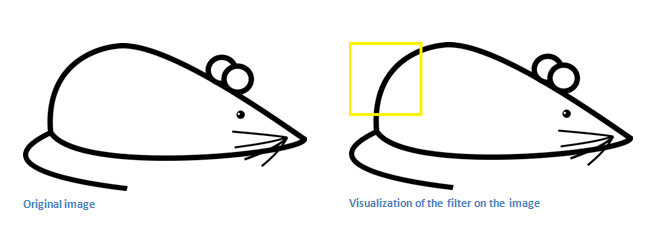
\includegraphics[width=10cm, keepaspectratio]{mouse}
\end{frame}

\begin{frame}{Examples}
	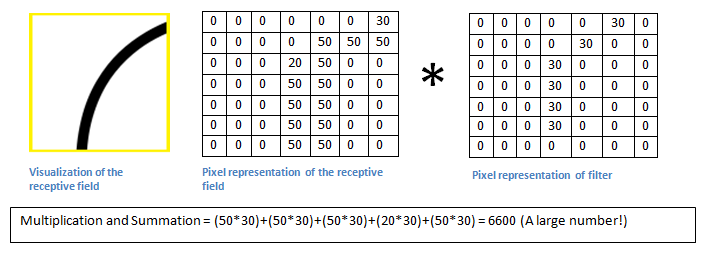
\includegraphics[width=10cm, keepaspectratio]{mousemult}
\end{frame}

\begin{frame}{Examples}
	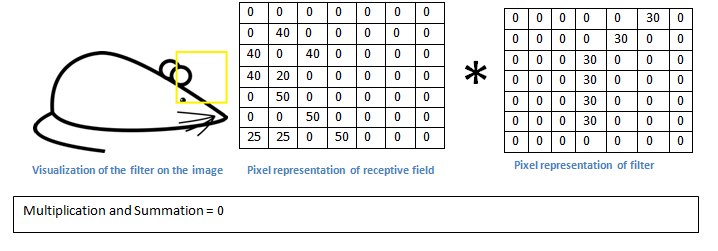
\includegraphics[width=10cm, keepaspectratio]{mousemult2}
\end{frame}


\begin{frame}{Max Pooling}
Down samples the volume spatially, independently in each depth slice of the input volume. 
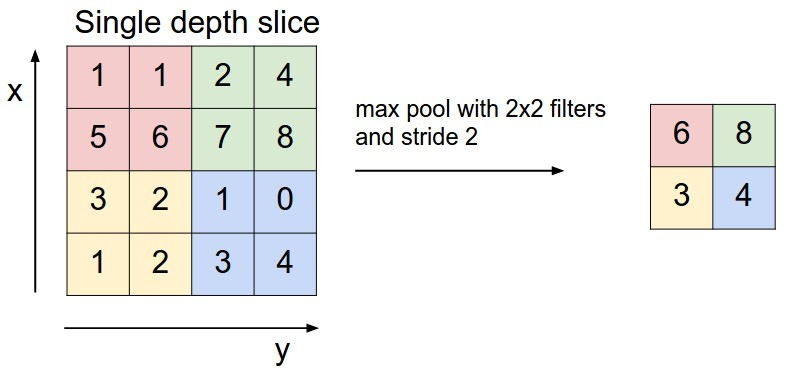
\includegraphics[width=10cm]{maxpool}
\end{frame}

\begin{frame}{Response Normalisation}
	ReLU (Rectified Linear Unit)
	$$f(x) = \max(0,x) $$
	\begin{itemize}
		\item Great speedup in training
		\item Simpler to compute than $\tanh$, sigmoid
		\item Can "die" if large gradient flows through then weight might update to prevent this neuron activating causing it to remain 0. We can prevent this by setting a proper learning rate or using Noisy ReLUs, Leaky ReLUL or 
	\end{itemize}

\end{frame}

\begin{frame}{Context}
	ImageNet
	\begin{itemize}
		\item 15 million labels images
		\item 22 thousand categories labeled by Amazon Mechanical Turk
	\end{itemize}
	ILSVRC
	\begin{itemize}
		\item Annual competition to classify images
		\item 1.2 million images and 1 thousand categories
		\item Top result and top 5 are considered
	\end{itemize}
\end{frame}



\begin{frame}{AlexNet}
By. Alex Krizhevsky, Ilya Sutskever, Geoffrey E. Hinton
\begin{itemize}
	\item Trained one of the largest (at the time) CNN's on the subset of ImageNet used for ILSVRC (Large Scale Recognition Challenge) and destroyed everyone else
	\item Wrote and published highly optimised GPU implementations of 2D convolution and other necessary operations
	\item New and unusual features that improve performance and reduce training time
	\item New techniques to prevent overfitting
	\item 5 convolution and 3 fully connected layers
	\item Size still limited by memory on GPUs at the time (they used 2x GTX 580's with 3GB VRAM each)
\end{itemize}
\end{frame}



\begin{frame}

	\begin{center}
		\Huge Architecture
	\end{center}
\end{frame}



\begin{frame}{ReLU Nonlinearity}
	\begin{itemize}
		\item Most people model neuron's output as $$f(x) = tanh(x)$$ or $$f(x)=(1+e^{-x})^{-1}$$
		\item When training with gradient descent these saturating nonlinearities are much slower than non-saturating nonlinearity
		\item Deep CNNs with ReLU train several times faster than $tanh$ networks
	\end{itemize}
	\begin{center}
		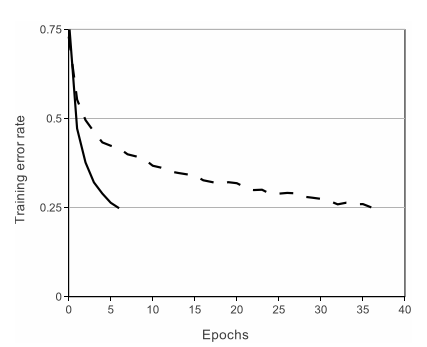
\includegraphics[width=5cm]{ReLU}
	\end{center}

\end{frame}


\begin{frame}{Mult GPU Training}
	\begin{itemize}
		\item The GTX580 that they trained on only had 3GB of memory, turns out 1.2 million images $>$ 3GB
		\item Spread the network across two GPUs as current GPUs are well suited to cross GPU parallelisation as they can read/write to each others memory without going through host
		\item Put half the kernels on each GPU, GPUs only communicate in certain layers 
	\end{itemize}
	
\let\thefootnote\relax\footnote{(how to get the University to pay for your sweet gaming rig)}
\end{frame}

\begin{frame}{Local Response Normalisation}
	\begin{itemize}
		\item ReLUs do not require input normalisation to prevent saturation, if at least one training examples gives positive input to ReLU learning happens
		\item Applying local normalisation aids generalisation 
		\item ReLU neurons have unbounded activations, we need to normalise this. We want to detect high frequency features with large response
		\item Normalising around the neighbourhood of excited neuron makes it more sensitive compared to neighbours
		\item Normalisation also dampens responses that are uniformly large in a given neighbourhood 
	\end{itemize}
\end{frame}



\begin{frame}{Overlapping Pooling}
	\begin{itemize}
		\item Pooling Layers summarise outputs of neighbouring pixels in the same kernel map
		\item Traditionally the neighbourhoods didn't overlap
		\item Overlapping pooling results in greater accuracy and slightly more difficulty overfitting 
	\end{itemize}
\end{frame}


\begin{frame}{Overall Architecture}
	\begin{itemize}
		\item 8 layers, first 5 are convolutional, last 3 fully connected
		\item Output of last fully connected layer is fed into 1000-way softmax which produced distribution over the 1000 class labels
		\item Networks maximises multinomial logistic regression objective, equivalent to maximising average across training cases of log-probability
	\end{itemize}
\end{frame}

\begin{frame}{Layers}
	Layer 1
	\begin{itemize}
		\item Input: $224\times 224\times 3$
		\item Kernels: 96 of size $11\times 11 \times 3$
		\item Stride 4 pixels (distance between centre of receptive fields
	\end{itemize}
	Layer 2
	\begin{itemize}
		\item Input: output of layer 1 after ReLU and max pooling
		\item Kernels: 256 of size $5\times 5 \times 48$
	\end{itemize}
	Layer 3
	\begin{itemize}
		\item Input: output of layer 2 after ReLU and max pooling
		\item Kernel: 384 of size $3\times 3\times 256$
	\end{itemize}
	
\end{frame}


\begin{frame}
	Layer 4
	\begin{itemize}
		\item Input: output of layer 3
		\item Kernel: 384 of size $3\times 3\times 192$ (note $192=\frac{384}{2}$ so the data didn't transfer between GPUs on this level)
	\end{itemize}
	Layer 5(last convolutional)
	\begin{itemize}
		\item Input: output of layer 3
		\item Kernels: 256 of size $3\times 3\times 192$ (note again no inter GPU transfer)
	\end{itemize}
\end{frame}

\begin{frame}{Altogether}
	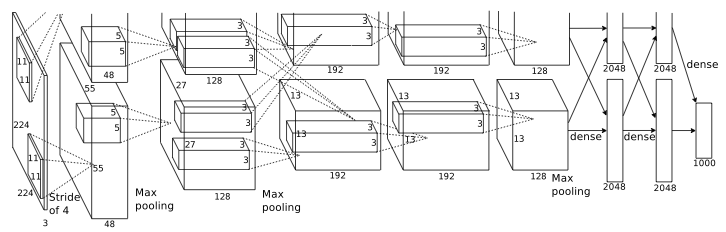
\includegraphics[width=10cm]{imagenet2GPU}
\end{frame}
\begin{frame}{Single GPU version}
	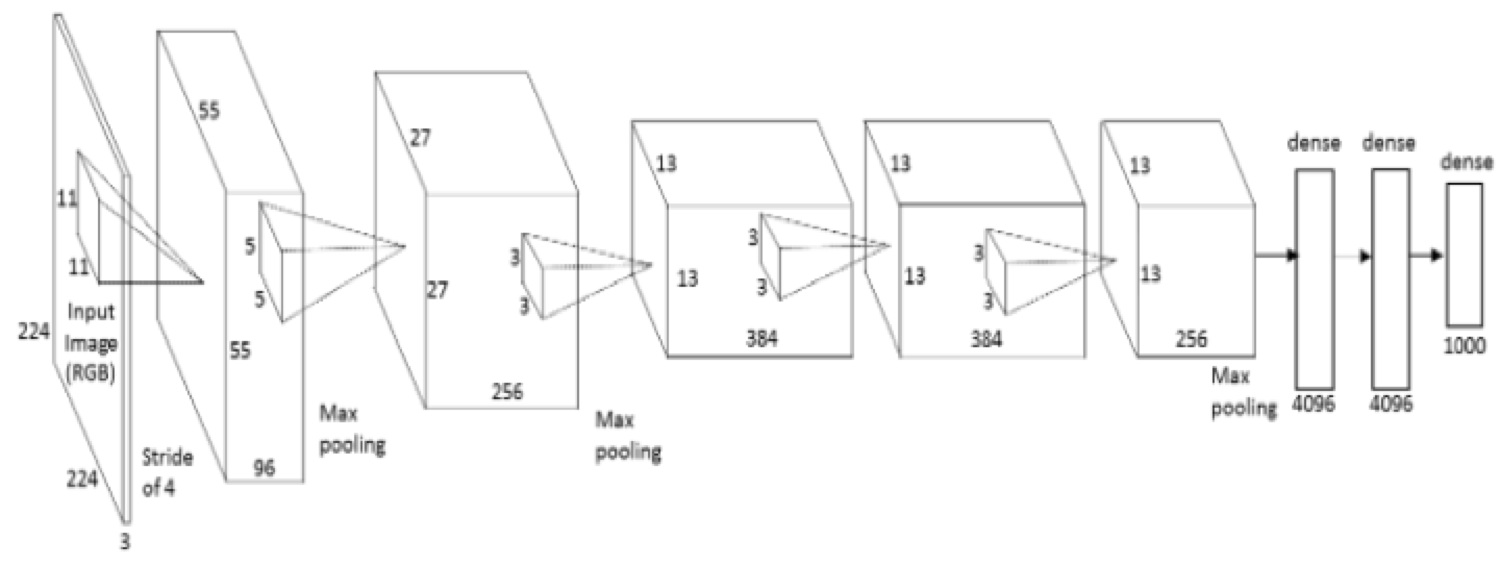
\includegraphics[width=10cm]{alexnet}
\end{frame}


\begin{frame}{Reducing Overfitting}
	\begin{itemize}
		\item Network has 60 million parameters, even with all the Imagenet data we can still easily overfit
	\end{itemize}
	Data Augmentation
	\begin{itemize}
		\item Artificially enlarge dataset using label preserving transforms
		\item Extract image and horizontal reflections. Image net images are $256\times 256$, AlexNet input is $224\times 224$
		\item this increases the input size by a factor of 2048 (although results are highly interdependent)
		\item Without this the network would substantially overfit thus requiring a smaller network
		\item At test time 5 $224\times 224$ patches are extracted (corners and centre) and their horizontal reflections
		\item We can also alternate the RGB values in the inputs
	\end{itemize}
\end{frame}


\begin{frame}{Dropout}
	\begin{itemize}
		\item Combining predictions of many models is a successful way to reduce test errors but is very expensive in big networks
		\item Dropout on the other hand only adds a factor of 2 to training time
		\item Dropout involves setting neurons to 0 during training with probability $0.5$
		\item Dropped neurons don't contribute in forward passes or backpropagation
		\item This results in a network that is different each time we pass in input data
		\item This reduces co-adaption of neurons (neurons doing the same thing) forcing learning of more robust features
	\end{itemize}
\end{frame}

\begin{frame}{Training Details}
	\begin{itemize}
		\item Trained using Stochastic Gradient Descent with batch size of 128, momentum 0.9, weight decay 0.0005
		\item Weight initialisation in each layer: zero mean Gaussian with $\sigma=0.01$
		\item Neuron bias in layers 2, 3, 4, 5 and fully connected initialised as 1
		\item This initialisation accelerates early learning as ReLU start with positive inputs
		\item Learning rate of 0.01, reduced by factor of 10 when validation rate stopped improving
		\item 90 cycles through 1.2 million images taking 5/6 days on 2 GTX580's
	\end{itemize}
\end{frame}

\begin{frame}{Results}
	\begin{itemize}
		\item top-1 error rate: 37.5%
		\item top-5 error rate: 17.0%
		\item Best performance on ILSVRC-2010 beating 47.1\% and 28.2\% respectively 	
	\end{itemize}
	\begin{center}
		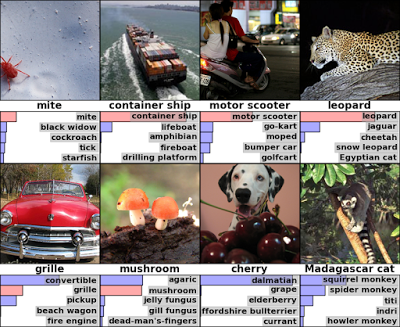
\includegraphics[width=6cm]{results}
	\end{center}
\end{frame}

\begin{frame}{Evaluating Convolutions}
	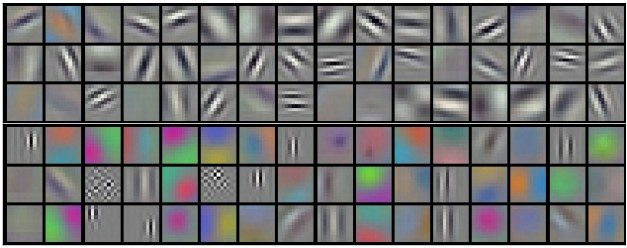
\includegraphics[width=10cm]{filters}\\
	Here's the 96 convolutional kernels of size $11\times 11\times 3$ from the first layer\\
	This shows the network has learned a variety of frequency and orientation selective kernels as well as colours blobs
\end{frame}

\begin{frame}{Evaluating Fully Connected Layers}
	\begin{center}
		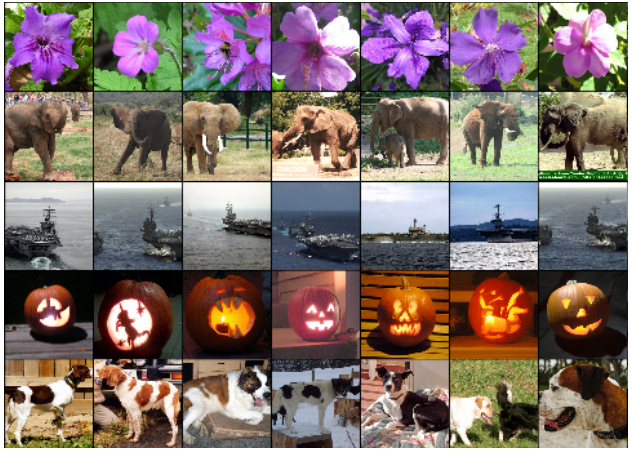
\includegraphics[width=8cm]{similar}\\
	\end{center}
	
	We can evaluate the fully connected layers by looking at images that excite the same collection of neurons\\
	Here we see rows of images that caused the same neurons to excite, showing the network segments images similarly internally
\end{frame}


\begin{frame}{Related further work}
	\begin{itemize}
		\item Dropout (Srivastava, Hinton, Krizhevsky, Sutkever, Slakhutdinov)
		\item VGGNet (Oxford Vision Group)
		\item Inception (Google)
		\item ResNet (Facebook)
	\end{itemize}
\end{frame}

\end{document}

              